\documentclass[11pt]{charter}

% El títulos de la memoria, se usa en la carátula y se puede usar el cualquier lugar del documento con el comando \ttitle
\titulo{Sistema de Aislamiento Limitado/Total Ferroviario} 

% Nombre del posgrado, se usa en la carátula y se puede usar el cualquier lugar del documento con el comando \degreename
\posgrado{Carrera de Especialización en Sistemas Embebidos} 
%\posgrado{Carrera de Especialización en Internet de las Cosas} 
%\posgrado{Carrera de Especialización en Intelegencia Artificial}
%\posgrado{Maestría en Sistemas Embebidos} 
%\posgrado{Maestría en Internet de las cosas}

% Tu nombre, se puede usar el cualquier lugar del documento con el comando \authorname
\autor{Ing. Nahuel Espinosa} 

% El nombre del director y co-director, se puede usar el cualquier lugar del documento con el comando \supname y \cosupname y \pertesupname y \pertecosupname
\director{Dr. Ing. Pablo Gomez}
\pertenenciaDirector{CONICET-GICSAFe} 
% FIXME:NO IMPLEMENTADO EL CODIRECTOR ni su pertenencia
\codirector{} % si queda vacio no se deberíá incluir 
\pertenenciaCoDirector{}

% Nombre del cliente, quien va a aprobar los resultados del proyecto, se puede usar con el comando \clientename y \empclientename
\cliente{}
\empresaCliente{}

% Nombre y pertenencia de los jurados, se pueden usar el cualquier lugar del documento con el comando \jurunoname, \jurdosname y \jurtresname y \perteunoname, \pertedosname y \pertetresname.
\juradoUno{Nombre y Apellido (1)}
\pertenenciaJurUno{pertenencia (1)} 
\juradoDos{Nombre y Apellido (2)}
\pertenenciaJurDos{pertenencia (2)}
\juradoTres{Nombre y Apellido (3)}
\pertenenciaJurTres{pertenencia (3)}
 
\fechaINICIO{22 de junio de 2020}		%Fecha de inicio de la cursada de GdP \fechaInicioName
\fechaFINALPlanificacion{22 de Agosto de 2020} 	%Fecha de final de cursada de GdP
\fechaFINALTrabajo{22 de diciembre de 2020}		%Fecha de defensa pública del trabajo final


\begin{document}

\maketitle
\thispagestyle{empty}
\pagebreak


\thispagestyle{empty}
{\setlength{\parskip}{0pt}
\tableofcontents{}
}
\pagebreak


\section{Registros de cambios}
\label{sec:registro}


\begin{table}[ht]
\label{tab:registro}
\centering

\begin{tabularx}{\linewidth}{@{}|c|X|c|@{}}
\hline
\rowcolor[HTML]{C0C0C0} 
Revisión & \multicolumn{1}{c|}{\cellcolor[HTML]{C0C0C0}Detalles de los cambios realizados} & Fecha      \\ \hline
1.0      & Creación del documento                                                          & 22/06/2020 \\ \hline
1.1      & Ejemplo de un texto muy largo que debiera ocupar más de una línea para que tengan de ejemplo                                                                                																						   & dd/mm/aaaa \\ \hline
1.2      & Otro ejemplo \newline
		   Con texto partido \newline
		   En varias líneas \newline
		   A propósito                                                                     & dd/mm/aaaa \\ \hline
\end{tabularx}
\end{table}

\pagebreak



\section{Acta de Constitución del Proyecto}
\label{sec:acta}

\begin{flushright}
Buenos Aires, \fechaInicioName
\end{flushright}

\vspace{2cm}

Por medio de la presente se acuerda con el \authorname\hspace{1px} que su Trabajo Final de la \degreename\hspace{1px} 
se titulará ``\ttitle'', consistirá esencialmente en el prototipo de un equipo que permita inhabilitar las señales de 
corte de tracción y frenado de emergencia en el caso de una falla en uno de los subsistemas de seguridad de una 
formación ferroviaria, y tendrá un presupuesto preliminar estimado de 600 hs de trabajo y \textcolor{red}{\$XXX}, con 
fecha de inicio \fechaInicioName\hspace{1px} y fecha de presentación pública \fechaFinalName.

Se adjunta a esta acta la planificación inicial.

\vfill

% Esta parte se construye sola con la información que hayan cargado en el preámbulo del documento y no debe modificarla
\begin{table}[ht]
\centering
\begin{tabular}{ccc}
\begin{tabular}[c]{@{}c@{}}Dr. Ing. Ariel Lutenberg \\ Director posgrado FIUBA\end{tabular} &  & \begin{tabular}[c]{@{}c@{}}\clientename \\ \empclientename \end{tabular} \vspace{2.5cm} \\ 
\multicolumn{3}{c}{\begin{tabular}[c]{@{}c@{}} \supname \\ Director del Trabajo Final\end{tabular}} \vspace{2.5cm} \\
\begin{tabular}[c]{@{}c@{}}\jurunoname \\ Jurado del Trabajo Final\end{tabular}     &  & \begin{tabular}[c]{@{}c@{}}\jurdosname\\ Jurado del Trabajo Final\end{tabular}  \vspace{2.5cm}  \\
\multicolumn{3}{c}{\begin{tabular}[c]{@{}c@{}} \jurtresname\\ Jurado del Trabajo Final\end{tabular}} \vspace{.5cm}                                                                     
\end{tabular}
\end{table}

\section{Descripción técnica-conceptual del Proyecto a realizar}
\label{sec:descripcion}

Las formaciones ferroviarias cuentan con diferentes sistemas de seguridad a bordo. Los mismos son equipos que se
encargan de supervisar el correcto funcionamiento de los subsistemas críticos. Ejemplos de los mismos son la seguridad
de puertas, el sistema de hombre vivo y la protección de coche a la deriva.

Ante una falla en uno de estos subsistemas, una formación ferroviaria se detiene inmediatamente por la activación 
automática de las señales de corte de tracción y frenado de emergencia. En esta situación el conductor debe llevar a la 
formación a un lugar seguro para que los pasajeros puedan descender y posteriormente a un taller para que pueda ser 
reparada.

En el año 2017, la empresa estatal Trenes Argentinos Operaciones (SOFSE) encargó al CONICET-GICSAFe el desarrollo de un 
equipo que le permita al conductor inhabilitar las señales de corte de tracción (CT) y frenado de emergencia (FE) sin comprometer 
la seguridad de la formación y sus pasajeros. Este equipo se conoce en el ámbito local como Sistema de Aislamiento 
Limitado/Total (SAL/T) y se considera un sistema crítico debido a que, en caso de fallar, puede 
ocasionar daños afectando negativamente la salud de las personas, al medio ambiente y/o generar grandes pérdidas 
materiales.

En el año 2019 se concluyó el desarrollo de un prototipo funcional del SAL/T  en el marco del trabajo de tesis del Ing. 
Ivan Di Vito. En la Figura \ref{fig:diagrama_de_bloques} se puede ver como interactúa con las señales CT y FE. En modo 
de funcionamiento normal los subsistemas de seguridad tienen conexión directa con el control central. Ante la activación 
por parte del conductor del modo aislado limitado (AL) el SAL/T toma el control de dichas señales.

\begin{figure}[htpb]
\centering 
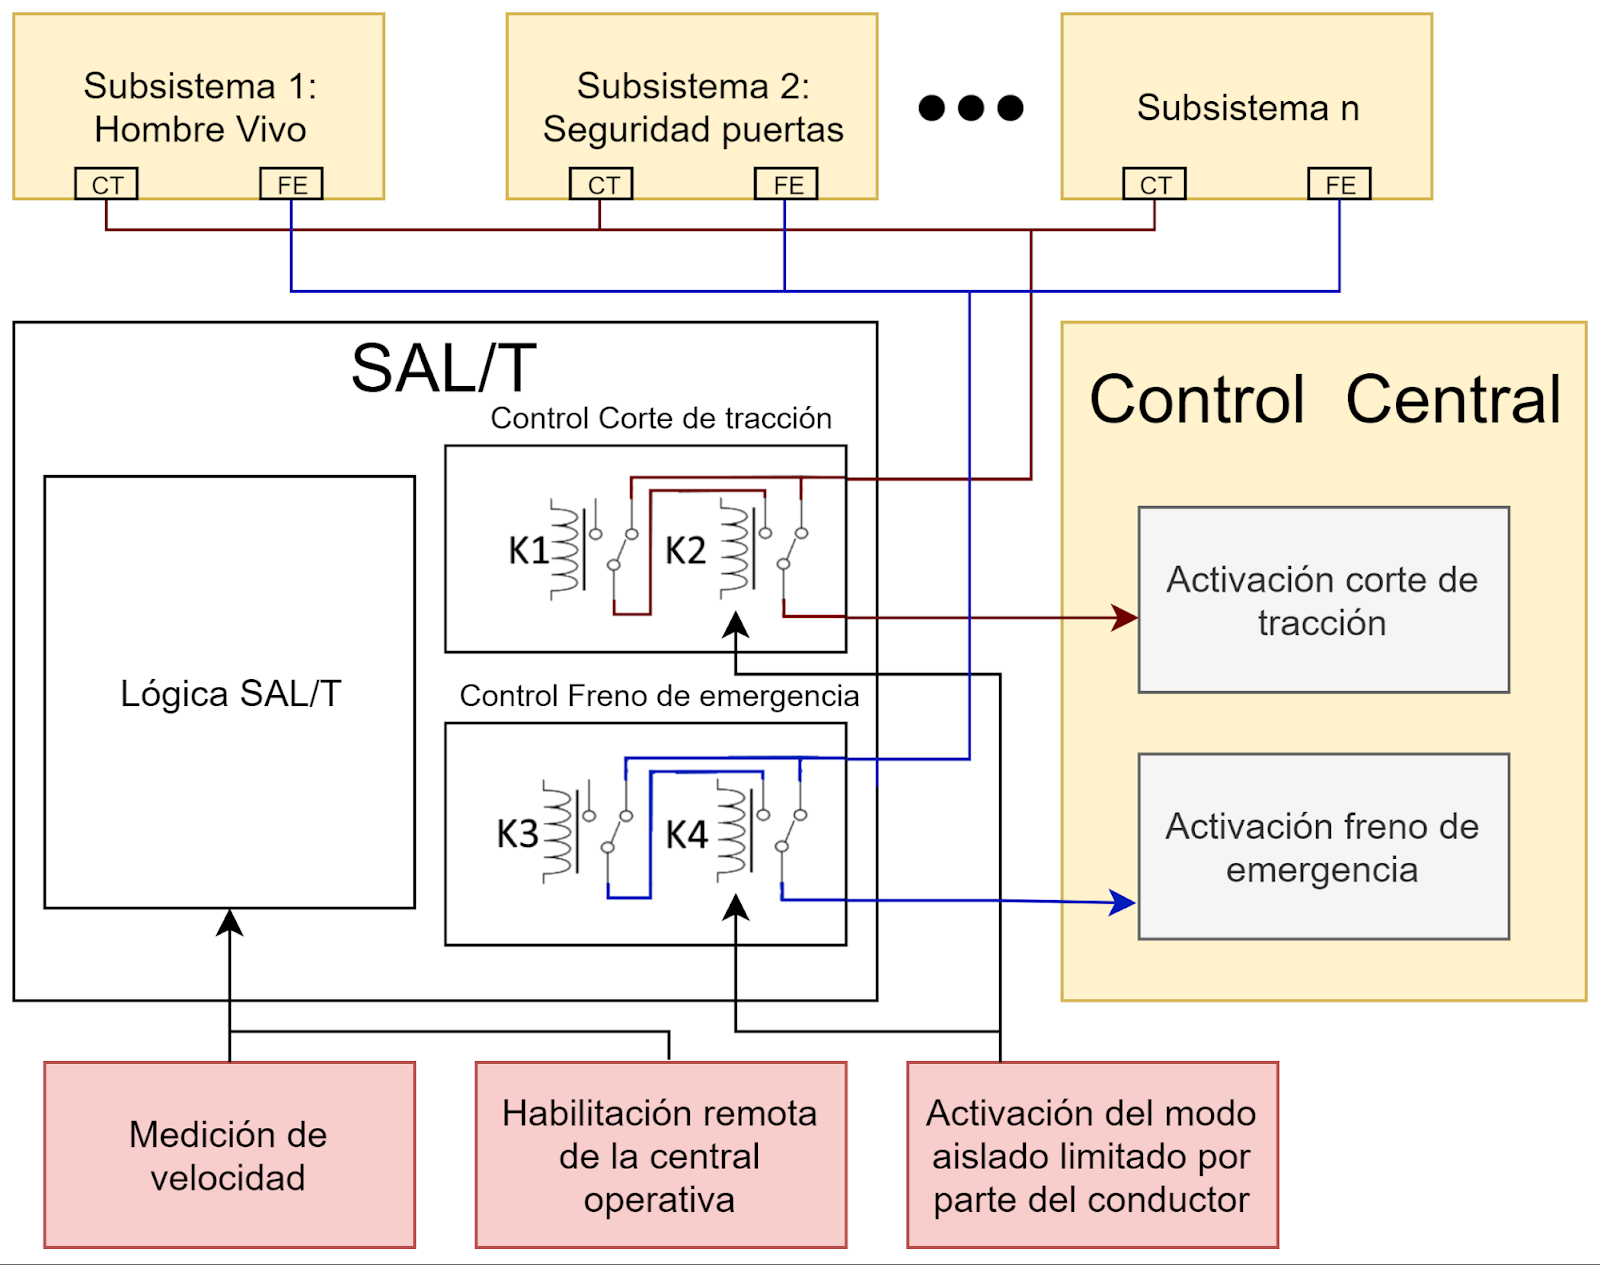
\includegraphics[width=.85\textwidth]{./Figuras/diagrama_de_bloques.png}
\caption{Diagrama conceptual de la interacción del SAL/T con los sistemas de seguridad en una formación.}
\label{fig:diagrama_de_bloques}
\end{figure}

El SAL/T monitorea la velocidad de la formación e informa su estado interno al registrador de eventos Hasler Teloc 1500 
y a una central operativa, a través de un enlace de comunicación redundado, de la cual también puede recibir comandos 
remotos que modifiquen su comportamiento.

En la Figura \ref{fig:ciclo_de_vida_50126} se resaltan las cinco primeras fases completadas del ciclo de vida propuesto 
por la norma UNE-EN 50126 para aplicaciones ferroviarias. La documentación de la sexta fase, que corresponde al diseño 
e implementación del sistema, y las fases posteriores quedaron fuera del alcance del trabajo original.

\vspace{10px}

\begin{figure}[htpb]
\centering 
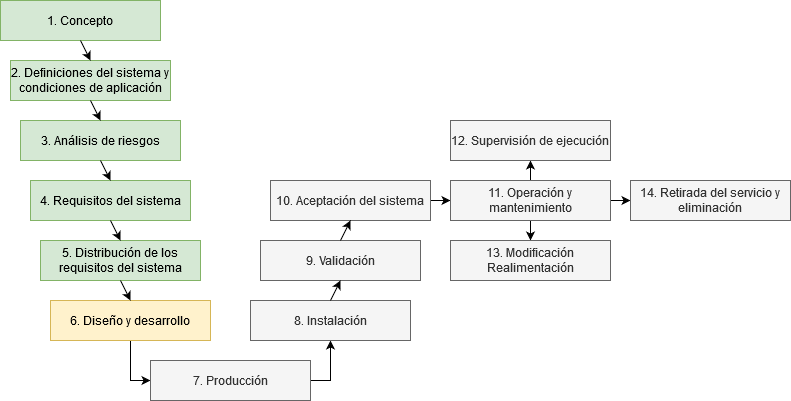
\includegraphics[width=1\textwidth]{./Figuras/ciclo_de_vida_50126.png}
\caption{Ciclo de vida de un sistema propuesto por la norma UNE-EN 50126.}
\label{fig:ciclo_de_vida_50126}
\end{figure}

\vspace{10px}

Este proyecto continuará con el desarrollo del SAL/T revisando los requisitos de seguridad RAMS establecidos en la cuarta fase 
del trabajo original, diseñando subsistemas que se ajusten a los requisitos y verificando el nivel de integridad 
de seguridad (SIL).

Para el caso específico de los sistemas eléctrico-programables (EP) la fase de diseño y desarrollo se divide en dos 
partes relacionadas con el desarrollo del hardware y del software.

\begin{itemize}
\item El diseño del software buscará seguir una metodología acorde a la norma UNE-EN 50128 centrada en la calidad de los 
aspectos de software de los sistemas de ferrocarriles.
\item En el nuevo diseño de la placa principal se reemplazará la plataforma EDU-CIAA-NXP, utilizada como base en la primera 
versión, por un módulo ad-hoc de procesamiento.
\end{itemize}

\newpage

\section{Identificación y análisis de los interesados}
\label{sec:interesados}

\begin{consigna}{red} 
Nota: (borrar esto y todas las consignas en color rojo antes de entregar este documento).
 
Es inusual que una misma persona esté en más de un rol, incluso en proyectos chicos.
 
Si se considera que una persona cumple dos o más roles, entonces sólo dejarla en el rol más importante. Por ejemplo:

\begin{itemize}
\item Si una persona es Cliente pero también colabora u orienta, dejarla solo como Cliente.
\item Si una persona es el Responsable, no debe ser colocado también como Miembro del equipo.
\end{itemize}

Pero en cambio sí es usual que el Cliente y el Auspiciante sean el mismo, por ejemplo.

\begin{table}[ht]
%\caption{Identificación de los interesados}
%\label{tab:interesados}
\begin{tabularx}{\linewidth}{@{}|l|X|X|l|@{}}
\hline
\rowcolor[HTML]{C0C0C0} 
Rol           & Nombre y Apellido & Organización 	& Puesto 	\\ \hline
Auspiciante   &                   &              	&        	\\ \hline
Cliente       & \clientename      &\empclientename	&        	\\ \hline
Impulsor      &                   &              	&        	\\ \hline
Responsable   & \authorname       & FIUBA        	& Alumno 	\\ \hline
Colaboradores &                   &              	&        	\\ \hline
Orientador    & \supname	      & \pertesupname 	& Director	Trabajo final \\ \hline
Equipo        & miembro1 \newline 
				miembro2          &              	&        	\\ \hline
Opositores    &                   &              	&        	\\ \hline
Usuario final &                   &              	&        	\\ \hline
\end{tabularx}
\end{table}

El Director suele ser uno de los Orientadores.

No dejar celdas vacías; si no hay nada que poner en una celda colocar un signo ``-''.

No dejar filas vacías; si no hay nada que poner en una fila entonces eliminarla.

Sería deseable listar a continuación de la tabla las principales características de cada interesado.
 
Por ejemplo:
\begin{itemize}
\item Auspiciante: es riguroso y exigente con la rendición de gastos. Tener mucho cuidado con esto.
\item Equipo: Juan Perez, suele pedir licencia porque tiene un familiar con una enfermedad. Planificar considerando esto.
\item Orientador: María Gómez, nos va a poder ayudar mucho con la gestión de impuestos.
\end{itemize}

\end{consigna}

\newpage

\section{1. Propósito del proyecto}
\label{sec:proposito}

El propósito de este proyecto es continuar el desarrollo de un sistema de supervisión de seguridad de formaciones ferroviarias 
denominado SAL/T (Sistema de Aislamiento Limitado/Total) que alcance niveles RAMS adecuados para su uso a criterio de las autoridades SOFSE y CNRT.

\section{2. Alcance del proyecto}
\label{sec:alcance}

El desarrollo del presente proyecto incluye:

\begin{itemize}
\item Revisión y actualización de la documentación generada en las primeras cinco fases del ciclo de vida del proyecto
original.
\item Diseño, implementación y documentación del firmware siguiendo la norma UNE-EN 50128 utilizando herramientas de integración y ensayos. 
\item Diseño y fabricación de una nueva versión de la placa principal del hardware reemplazando la EDU-CIAA-NXP por un procesador ad-hoc.
\item Verificación del nivel de integridad de seguridad (SIL) del sistema.
\end{itemize}

El presente proyecto NO incluye:

\begin{itemize}
\item Desarrollo de la séptima fase y posteriores del ciclo de vida del proyecto (producción, instalación, validación, etc.).
\item Desarrollo del software necesario para la central operativa.
\item Modificación del gabinete.
\item Certificación de los sistemas a ser desarrollados.
\end{itemize}

\section{3. Supuestos del proyecto}
\label{sec:supuestos}

Para el desarrollo del presente proyecto se supone que:

\begin{itemize}
\item El análisis, la definición de subsistemas, interacciones y uso de patrones de diseño en el trabajo original seguirán 
siendo válidos para la segunda iteración del proyecto.
\item Se tendrá acceso al prototipo actual para hacer pruebas de integridad con el nuevo firmware.
\item Una vez finalizado el diseño del PCB, se podrá fabricar el mismo en un tiempo razonable. 
\item No habrá dificultades para conseguir los componentes electrónicos necesarios.
\item Se adquirirán los conocimientos necesarios sobre la normativa aplicable.
\item El tiempo estipulado será suficiente para alcanzar los objetivos definidos.
\end{itemize}

\section{4. Requerimientos}
\label{sec:requerimientos}

Estos requerimientos fueron obtenidos a partir del documento ''R\_DCP\_10 Definición Conceptual del Proyecto - Fase 1''. El mismo
fue creado originalmente por el Ing. Ivan Di Vito siguiendo la recomendación de la norma UNE-EN 50126 como resultado de múltiples 
reuniones con las diferentes partes interesadas en la realización del proyecto. 

Esas reuniones incluyeron la participación de personal de SOFSE de la Gerencia
de Seguridad Operacional, del departamento de material rodante y de personal de los talleres de reparación y mantenimiento
de Liniers y Victoria. También participó personal de la Comisión Nacional de Regulación del Transporte (CNRT).

Se estudió la documentación original teniendo en cuenta el estado actual del prototipo y se redactaron los requerimientos
agrupándolos por afinidad:

\begin{enumerate}
\item Grupo de requerimientos asociados al modo normal de funcionamiento
  \begin{enumerate}
  \item No debe intervenir en el funcionamiento del material rodante (prioridad alta).
  \item Debe obtener en todo momento la mejor estimación posible de la velocidad de la formación.
    \begin{enumerate}
    \item Debe ser capaz de recibir la velocidad a partir de una señal digital provista por el registrador de eventos Hasler Teloc 1500.
    \item Debe ser capaz de calcular la velocidad a partir de un generador de impulsos ópticos instalado en una o varias ruedas de la formación.
    \item Debe ser capaz de calcular la velocidad a partir de un sistema GPS integrado.
    \end{enumerate}
  \item El rango de velocidad soportado por el sistema tiene que estar entre 0 y 120 km/h.
  \item La estimación de velocidad debe tener una precisión del 2\% de fondo de escala. 
  \end{enumerate}
\item Grupo de requerimientos asociados al modo aislado limitado
  \begin{enumerate}
  \item Debe evitar la aplicación del corte de tracción y/o freno de emergencia por parte de los subsistemas de seguridad del material rodante.
  \item Debe emitir una señal sonora intermitente a través de un buzzer.
  \item Debe evitar que la velocidad del material rodante supere una serie de límites configurados.
    \begin{enumerate}
    \item Si al pasar de modo normal a modo aislado limitado no se cuenta con una estimación de velocidad, debe activar el corte de tracción y el freno de emergencia por 30 segundos.
    \item Si se supera una velocidad configurable (por defecto 30 km/h), debe activar el corte de tracción y emitir una señal sonora continua a través de un buzzer.
    \item Si se supera una velocidad configurable (por defecto 36 km/h), debe activar el freno de emergencia.
    \item Una vez aplicado, el corte de tracción debe dejar de aplicarse si la velocidad vuelve a ser menor a una velocidad configurable (por defecto 25 km/h). 
    \item Una vez aplicado, el freno de emergencia sólo debe dejar de aplicarse luego de un tiempo configurable (por defecto 30 segundos) desde que se superó el límite.
    \item Si la lectura de velocidad es inválida, debe activar y desactivar el corte de tracción y freno de emergencia de manera alternada en ciclos de tiempo configurables.
    \end{enumerate}
  \end{enumerate}
\newpage
\item Grupo de requerimientos asociados con la interfaz humano-máquina
  \begin{enumerate}
  \item Debe contar con una llave rotativa precintable para activar el modo aislado limitado.
  \item Debe indicar el estado del sistema.
  \item Debe mostrar la velocidad media del equipo en km/h (3 ó 4 dígitos).
  \item Debe indicar el estado de las señales de corte de tracción y freno de emergencia.
  \item Debe indicar la presencia de un comando remoto de la central operativa.
  \item Debe indicar el estado de los módulos GPS.
  \end{enumerate}
\item Grupo de requerimientos asociados con las comunicaciones
  \begin{enumerate}
    \item Debe informar al registrador de eventos la activación del modo aislado limitado.
    \item Debe informar al registrador de eventos si la alimentación es correcta.
    \item Debe informar al registrador de eventos la activación del freno de emergencia.
    \item Debe informar al registrador de eventos la activación del corte de tracción.
    \item Debe informar periódicamente el estado del sistema a la central operativa a través de la red de datos GPRS/3G/4G.
    \item Debe existir la posibilidad de usar 2 proveedores distintos de datos de manera simultánea.
    \item El protocolo de comunicación con la central operativa debe ser MQTT.
    \item Debe ser capaz de recibir un comando remoto que anule el corte de tracción y el freno de emergencia bajo cualquier condición (modo aislado total).
    \item Debe ser capaz de recibir un comando remoto que active el corte de tracción y el freno de emergencia bajo cualquier condición (modo parada total).
    \item Debe ser capaz de recibir un comando remoto que active el corte de tracción y anule el freno de emergencia bajo cualquier condición (modo coche en deriva).
    \item Debe ser capaz de recibir un comando remoto que active el corte de tracción y el freno de emergencia de forma intermitente en ciclos de tiempo configurables (modo intermitente).
    \item Debe ser capaz de recibir un comando remoto que cancele cualquier comando remoto vigente (exit). 
    \item Debe ser capaz de recibir comandos remotos que modifiquen sus parámetros internos configurables.
    \item Si no recibe un nuevo comando remoto luego de un tiempo configurable (por defecto 10 segundos, máximo 1 minuto), debe volver al algoritmo de activación de corte de tracción y freno de emergencia por defecto.
    \item Ante un comando remoto recibido debe enviar una confirmación de recepción que permita a la central operativa decidir si es necesaria o no una retransmisión.
    \item Debe utilizar algún mecanismo de encriptación para el enlace con la central operativa.
  \end{enumerate}
\item Grupo de requerimientos asociados al hardware y al gabinete
  \begin{enumerate}
    \item La tensión nominal de alimentación debe estar comprendida entre 72 V y 120 V.
    \item Los conectores deben ser unívocos imposibilitando la conexión incorrecta.
    \item Debe poseer una única placa para el procesamiento principal.
    \item Debe estar diseñado para ser instalado en la locomotora sobre el pupitre.
    \item El gabinete debe tener grado de seguridad IP66 o superior.
  \end{enumerate}
\end{enumerate}


\section{5. Entregables principales del proyecto}
\label{sec:entregables}

\begin{consigna}{red}
Cosas como: 
\begin{itemize}
\item Manual de uso
\item Diagrama esquemático
\item Código fuente
\item Diagrama de instalación
\item Informe final

\end{itemize}

\end{consigna}

\section{6. Desglose del trabajo en tareas}
\label{sec:wbs}

\begin{consigna}{red}
Se recomienda mostrar el WBS mediante una lista indexada:

\begin{enumerate}
\item Grupo de tareas 1
	\begin{enumerate}
	\item Tarea 1 (tantas hs)
	\item Tarea 2 (tantas hs)
	\item Tarea 3 (tantas hs)
	\end{enumerate}
\item Grupo de tareas 2
	\begin{enumerate}
	\item Tarea 1 (tantas hs)
	\item Tarea 2 (tantas hs)
	\item Tarea 3 (tantas hs)
	\end{enumerate}
	\item Grupo de tareas 3
	\begin{enumerate}
	\item Tarea 1 (tantas hs)
	\item Tarea 2 (tantas hs)
	\item Tarea 3 (tantas hs)
	\item Tarea 4 (tantas hs)
	\item Tarea 5 (tantas hs)
	\end{enumerate}
\end{enumerate}

Cantidad total de horas: (tantas hs)

Se recomienda que no haya ninguna tarea que lleve más de 40 hs. 

\end{consigna}

\section{7. Diagrama de Activity On Node}
\label{sec:AoN}

\begin{consigna}{red}
Armar el AoN a partir del WBS definido en la etapa anterior. 

%La figura \ref{fig:AoN} fue elaborada con el paquete latex tikz y pueden consultar la siguiente referencia \textit{online}:

%\url{https://www.overleaf.com/learn/latex/LaTeX_Graphics_using_TikZ:_A_Tutorial_for_Beginners_(Part_3)\%E2\%80\%94Creating_Flowcharts}

\end{consigna}

\begin{figure}[htpb]
\centering 
\includegraphics[width=.8\textwidth]{./Figuras/AoN.png}
\caption{Diagrama en \textit{Activity on Node}}
\label{fig:AoN}
\end{figure}

\begin{consigna}{red}

Indicar claramente en qué unidades están expresados los tiempos.
De ser necesario indicar los caminos semicríticos y analizar sus tiempos mediante un cuadro.
Es recomendable usar colores y un cuadro indicativo describiendo qué representa cada color, como se muestra en el siguiente ejemplo:

\end{consigna}

\section{8. Diagrama de Gantt}
\label{sec:gantt}

\begin{consigna}{red}
Utilizar el software Gantter for Google Drive o alguno similar para dibujar el diagrama de Gantt.

Existen muchos programas y recursos \textit{online} para hacer diagramas de gantt, entre las cuales destacamos:

\begin{itemize}
\item Planner
\item GanttProject
\item Trello + \textit{plugins}. En el siguiente link hay un tutorial oficial: \\ \url{https://blog.trello.com/es/diagrama-de-gantt-de-un-proyecto}
\item Creately, herramienta online colaborativa. \\\url{https://creately.com/diagram/example/ieb3p3ml/LaTeX}
\item Se puede hacer en latex con el paquete \textit{pgfgantt}\\ \url{http://ctan.dcc.uchile.cl/graphics/pgf/contrib/pgfgantt/pgfgantt.pdf}
\end{itemize}

Pegar acá una captura de pantalla del diagrama de Gantt, cuidando que la letra sea suficientemente grande como para ser legible. 
Si el diagrama queda demasiado ancho, se puede pegar primero la ``tabla'' del Gantt y luego pegar la parte del diagrama de barras del diagrama de Gantt.

Configurar el software para que en la parte de la tabla muestre los códigos del EDT (WBS).\\
Configurar el software para que al lado de cada barra muestre el nombre de cada tarea.\\
Revisar que la fecha de finalización coincida con lo indicado en el Acta Constitutiva.

En la figura \ref{fig:gantt}, se muestra un ejemplo de diagrama de gantt realizado con el paquete de \textit{pgfgantt}. En la plantilla pueden ver el código que lo genera y usarlo de base para construir el propio.

\begin{figure}[htbp]
\begin{center}
\begin{ganttchart}{1}{12}
  \gantttitle{2020}{12} \\
  \gantttitlelist{1,...,12}{1} \\
  \ganttgroup{Group 1}{1}{7} \\
  \ganttbar{Task 1}{1}{2} \\
  \ganttlinkedbar{Task 2}{3}{7} \ganttnewline
  \ganttmilestone{Milestone o hito}{7} \ganttnewline
  \ganttbar{Final Task}{8}{12}
  \ganttlink{elem2}{elem3}
  \ganttlink{elem3}{elem4}
\end{ganttchart}
\end{center}
\caption{Diagrama de gantt de ejemplo}
\label{fig:gantt}
\end{figure}

\end{consigna}

\section{9. Matriz de uso de recursos de materiales}
\label{sec:recursos}


\begin{table}[htpb]
\label{tab:recursos}
\centering
\begin{tabularx}{\linewidth}{@{}|c|X|X|X|X|X|@{}}
\hline
\cellcolor[HTML]{C0C0C0} & \cellcolor[HTML]{C0C0C0} & \multicolumn{4}{c|}{\cellcolor[HTML]{C0C0C0}Recursos requeridos (horas)} \\ \cline{3-6} 
\multirow{-2}{*}{\cellcolor[HTML]{C0C0C0}\begin{tabular}[c]{@{}c@{}}Código\\ WBS\end{tabular}} & \multirow{-2}{*}{\cellcolor[HTML]{C0C0C0}\begin{tabular}[c]{@{}c@{}}Nombre \\ tarea\end{tabular}} & Material 1 & Material 2 & Material 3 & Material 4 \\ \hline
 &  &  &  &  &  \\ \hline
 &  &  &  &  &  \\ \hline
 &  &  &  &  &  \\ \hline
 &  &  &  &  &  \\ \hline
\end{tabularx}%
\end{table}


\section{10. Presupuesto detallado del proyecto}
\label{sec:presupuesto}

\begin{consigna}{red}
Si el proyecto es complejo entonces separarlo en partes:
\begin{itemize}
\item Un total global, indicando el subtotal acumulado por cada una de las áreas.
\item El desglose detallado del subtotal de cada una de las áreas.
\end{itemize}

IMPORTANTE: No olvidarse de considerar los COSTOS INDIRECTOS.

\end{consigna}

\begin{table}[htpb]
\centering
\begin{tabularx}{\linewidth}{@{}|X|c|r|r|@{}}
\hline
\rowcolor[HTML]{C0C0C0} 
\multicolumn{4}{|c|}{\cellcolor[HTML]{C0C0C0}COSTOS DIRECTOS} \\ \hline
\rowcolor[HTML]{C0C0C0} 
Descripción &
  \multicolumn{1}{c|}{\cellcolor[HTML]{C0C0C0}Cantidad} &
  \multicolumn{1}{c|}{\cellcolor[HTML]{C0C0C0}Valor unitario} &
  \multicolumn{1}{c|}{\cellcolor[HTML]{C0C0C0}Valor total} \\ \hline
 &
  \multicolumn{1}{c|}{} &
  \multicolumn{1}{c|}{} &
  \multicolumn{1}{c|}{} \\ \hline
 &
  \multicolumn{1}{c|}{} &
  \multicolumn{1}{c|}{} &
  \multicolumn{1}{c|}{} \\ \hline
\multicolumn{1}{|l|}{} &
   &
   &
   \\ \hline
\multicolumn{1}{|l|}{} &
   &
   &
   \\ \hline
\multicolumn{3}{|c|}{SUBTOTAL} &
  \multicolumn{1}{c|}{} \\ \hline
\rowcolor[HTML]{C0C0C0} 
\multicolumn{4}{|c|}{\cellcolor[HTML]{C0C0C0}COSTOS INDIRECTOS} \\ \hline
\rowcolor[HTML]{C0C0C0} 
Descripción &
  \multicolumn{1}{c|}{\cellcolor[HTML]{C0C0C0}Cantidad} &
  \multicolumn{1}{c|}{\cellcolor[HTML]{C0C0C0}Valor unitario} &
  \multicolumn{1}{c|}{\cellcolor[HTML]{C0C0C0}Valor total} \\ \hline
\multicolumn{1}{|l|}{} &
   &
   &
   \\ \hline
\multicolumn{1}{|l|}{} &
   &
   &
   \\ \hline
\multicolumn{1}{|l|}{} &
   &
   &
   \\ \hline
\multicolumn{3}{|c|}{SUBTOTAL} &
  \multicolumn{1}{c|}{} \\ \hline
\rowcolor[HTML]{C0C0C0}
\multicolumn{3}{|c|}{TOTAL} &
   \\ \hline
\end{tabularx}%
\end{table}


\section{11. Matriz de asignación de responsabilidades}
\label{sec:responsabilidades}
\begin{consigna}{red}
Establecer la matriz de asignación de responsabilidades y el manejo de la autoridad completando la siguiente tabla:

\begin{table}[htpb]
\centering
\resizebox{\textwidth}{!}{%
\begin{tabular}{|c|c|c|c|c|c|}
\hline
\rowcolor[HTML]{C0C0C0} 
\cellcolor[HTML]{C0C0C0} &
  \cellcolor[HTML]{C0C0C0} &
  \multicolumn{4}{c|}{\cellcolor[HTML]{C0C0C0}Listar todos los nombres y roles del proyecto} \\ \cline{3-6} 
\rowcolor[HTML]{C0C0C0} 
\cellcolor[HTML]{C0C0C0} &
  \cellcolor[HTML]{C0C0C0} &
  Responsable &
  Orientador &
  Equipo &
  Cliente \\ \cline{3-6} 
\rowcolor[HTML]{C0C0C0} 
\multirow{-3}{*}{\cellcolor[HTML]{C0C0C0}\begin{tabular}[c]{@{}c@{}}Código\\ WBS\end{tabular}} &
  \multirow{-3}{*}{\cellcolor[HTML]{C0C0C0}Nombre de la tarea} &
  \authorname &
  \supname &
  Nombre de alguien &
  \clientename \\ \hline
 &  &  &  &  &  \\ \hline
 &  &  &  &  &  \\ \hline
 &  &  &  &  &  \\ \hline
\end{tabular}%
}
\end{table}

{\footnotesize
Referencias:
\begin{itemize}
	\item P = Responsabilidad Primaria
	\item S = Responsabilidad Secundaria
	\item A = Aprobación
	\item I = Informado
	\item C = Consultado
\end{itemize}
} %footnotesize

Una de las columnas debe ser para el Director, ya que se supone que participará en el proyecto.
A su vez se debe cuidar que no queden muchas tareas seguidas sin ``A'' o ``I''.

Importante: es redundante poner ``I/A'' o ``I/C'', porque para aprobarlo o responder consultas primero la persona debe ser informada.

\end{consigna}

\section{12. Gestión de riesgos}
\label{sec:riesgos}

\begin{consigna}{red}
a) Identificación de los riesgos (al menos cinco) y estimación de sus consecuencias:
 
Riesgo 1: detallar el riesgo (riesgo es algo que si ocurre altera los planes previstos)
\begin{itemize}
\item Severidad (S): mientras más severo, más alto es el número (usar números del 1 al 10).\\
Justificar el motivo por el cual se asigna determinado número de severidad (S).
\item Probabilidad de ocurrencia (O): mientras más probable, más alto es el número (usar del 1 al 10).\\
Justificar el motivo por el cual se asigna determinado número de (O). 
\end{itemize}   

Riesgo 2:
\begin{itemize}
\item Severidad (S): 
\item Ocurrencia (O):
\end{itemize}

Riesgo 3:
\begin{itemize}
\item Severidad (S): 
\item Ocurrencia (O):
\end{itemize}


b) Tabla de gestión de riesgos:      (El RPN se calcula como RPN=SxO)

\begin{table}[htpb]
\centering
\begin{tabularx}{\linewidth}{@{}|X|c|c|c|c|c|c|@{}}
\hline
\rowcolor[HTML]{C0C0C0} 
Riesgo & S & O & RPN & S* & O* & RPN* \\ \hline
       &   &   &     &    &    &      \\ \hline
       &   &   &     &    &    &      \\ \hline
       &   &   &     &    &    &      \\ \hline
       &   &   &     &    &    &      \\ \hline
       &   &   &     &    &    &      \\ \hline
\end{tabularx}%
\end{table}

Criterio adoptado: 
Se tomarán medidas de mitigación en los riesgos cuyos números de RPN sean mayores a ....

Nota: los valores marcados con (*) en la tabla corresponden luego de haber aplicado la mitigación.

c) Plan de mitigación de los riesgos que originalmente excedían el RPN máximo establecido:
 
Riesgo 1: Plan de mitigación (si por el RPN fuera necesario elaborar un plan de mitigación).
  Nueva asignación de S y O, con su respectiva justificación:
  - Severidad (S): mientras más severo, más alto es el número (usar números del 1 al 10).
          Justificar el motivo por el cual se asigna determinado número de severidad (S).
  - Probabilidad de ocurrencia (O): mientras más probable, más alto es el número (usar del 1 al 10).
          Justificar el motivo por el cual se asigna determinado número de (O).

Riesgo 2: Plan de mitigación (si por el RPN fuera necesario elaborar un plan de mitigación).
 
Riesgo 3: Plan de mitigación (si por el RPN fuera necesario elaborar un plan de mitigación)

\end{consigna}


\section{13. Gestión de la calidad}
\label{sec:calidad}

\begin{consigna}{red}
Para cada uno de los requerimientos del proyecto indique:
\begin{itemize} 
\item Req \#1: Copiar acá el requerimiento.

Verificación y validación:

\begin{itemize}
\item Verificación para confirmar si se cumplió con lo requerido antes de mostrar el sistema al cliente:\\
Detallar 
\item Validación con el cliente para confirmar que está de acuerdo en que se cumplió con lo requerido:\\
Detallar  
\end{itemize}

\end{itemize}

Tener en cuenta que en este contexto se pueden mencionar simulaciones, cálculos, revisión de hojas de datos, consulta con expertos, etc.

\end{consigna}

\section{14. Comunicación del proyecto}
\label{sec:comunicaciones}

\begin{consigna}{red}
El plan de comunicación del proyecto es el siguiente:
\end{consigna}

% Please add the following required packages to your document preamble:
% \usepackage{graphicx}
% \usepackage[table,xcdraw]{xcolor}
% If you use beamer only pass "xcolor=table" option, i.e. \documentclass[xcolor=table]{beamer}
\begin{table}[htpb]
\centering
\resizebox{\textwidth}{!}{%
\begin{tabular}{|c|c|c|c|c|c|}
\hline
\rowcolor[HTML]{C0C0C0} 
\multicolumn{6}{|c|}{\cellcolor[HTML]{C0C0C0}PLAN DE COMUNICACIÓN DEL PROYECTO}           \\ \hline
\rowcolor[HTML]{C0C0C0} 
¿Qué comunicar? & Audiencia & Propósito & Frecuencia & Método de comunicac. & Responsable \\ \hline
                &           &           &            &                      &             \\ \hline
                &           &           &            &                      &             \\ \hline
                &           &           &            &                      &             \\ \hline
                &           &           &            &                      &             \\ \hline
                &           &           &            &                      &             \\ \hline
\end{tabular}%
}
\end{table}

\section{15. Gestión de Compras}
\label{sec:compras}

\begin{consigna}{red}
En caso de tener que comprar elementos o contratar servicios:
a) Explique con qué criterios elegiría a un proveedor.
b) Redacte el Statement of Work correspondiente.
\end{consigna}

\section{16. Seguimiento y control}
\label{sec:seguimiento}

\begin{consigna}{red}
Para cada tarea del proyecto establecer la frecuencia y los indicadores con los se seguirá su avance y quién será el responsable de hacer dicho seguimiento y a quién debe comunicarse la situación (en concordancia con el Plan de Comunicación del proyecto).

El indicador de avance tiene que ser algo medible, mejor incluso si se puede medir en \% de avance. Por ejemplo,se pueden indicar en esta columna cosas como ``cantidad de conexiones ruteadeas'' o ``cantidad de funciones implementadas'', pero no algo genérico y ambiguo como ``\%'', porque el lector no sabe porcentaje de qué cosa.

\end{consigna}

\begin{table}[!htpb]
\centering
\begin{tabularx}{\linewidth}{@{}|X|X|X|X|X|X|@{}}
\hline
\rowcolor[HTML]{C0C0C0} 
\multicolumn{6}{|c|}{\cellcolor[HTML]{C0C0C0}SEGUIMIENTO DE AVANCE}                                                                       \\ \hline
\rowcolor[HTML]{C0C0C0} 
Tarea del WBS & Indicador de avance & Frecuencia de reporte & Resp. de seguimiento & Persona a ser informada & Método de comunic. \\ \hline
 &  &  &  &  &  \\ \hline
 &  &  &  &  &  \\ \hline
 &  &  &  &  &  \\ \hline
 &  &  &  &  &  \\ \hline
 &  &  &  &  &  \\ \hline
\end{tabularx}%
%}
\end{table}

\section{17. Procesos de cierre}    
\label{sec:cierre}

\begin{consigna}{red}
Establecer las pautas de trabajo para realizar una reunión final de evaluación del proyecto, tal que contemple las siguientes actividades:

\begin{itemize}
\item Pautas de trabajo que se seguirán para analizar si se respetó el Plan de Proyecto original:
 - Indicar quién se ocupará de hacer esto y cuál será el procedimiento a aplicar. 
\item Identificación de las técnicas y procedimientos útiles e inútiles que se utilizaron, y los problemas que surgieron y cómo se solucionaron:
 - Indicar quién se ocupará de hacer esto y cuál será el procedimiento para dejar registro.
\item Indicar quién organizará el acto de agradecimiento a todos los interesados, y en especial al equipo de trabajo y colaboradores:
  - Indicar esto y quién financiará los gastos correspondientes.
\end{itemize}

\end{consigna}


\end{document}
